\input{../preamble.tex}

\lecturenumber{7}
\title{Scheduling: The Switching Mechanism}
\version{2.0.0}

\begin{document}

\begin{frame}[plain, noframenumbering]
    \titlepage
\end{frame}

\begin{slide}

    \slidetitle{How does the OS run a process?}
    
    \begin{minipage}{0.5\textwidth}
    1. OS creates PCB
    \medskip
    
    2. OS allocates memory
    \medskip
    
    3. OS initializes registers
    
    \bigskip
    4. Process is in ready state
    \medskip
    
    5. When the process runs, the process executes directly on CPU
    
    \bigskip
    There is a transfer of CPU ownership
    \end{minipage}
    
\end{slide}

\begin{slide}

    \slidetitle{How Does the OS Switch Between Processes?}
    
    A process has the ownership of the CPU when it runs.
    \bigskip
    
    To switch to a different process, the OS needs to regain control.

\end{slide}

\begin{slide}

    \slidetitle{Aside: A simple function call}

    \begin{minipage}{0.5\textwidth}
    A new stack frame is pushed to the stack and the SP updated.
    \bigskip
    
    The old PC pushed to the stack and updated.
    \end{minipage}
    
\end{slide}

\begin{slide}

    \slidetitle{How about a system call?}
    
    The OS provides user programs with controlled access to system functionality.
    \bigskip
    
    \texttt{write()}
    \medskip
    
    \texttt{fork()}
    \medskip
    
    \texttt{pipe()}
    \bigskip
    
    How is a system call different from a function call?
    
\end{slide}

\begin{slide}

    \slidetitle{How about a system call?}
    
    CPU hardware has multiple privilege levels
    \begin{itemize}
        \item One to run user code: user mode
        \item One to run OS code like system calls: kernel mode
        \item Some instructions execute only in kernel mode
    \end{itemize}
    \bigskip
    
    Kernel does not trust user stack
    \begin{itemize}
        \item Uses a separate kernel stack when in kernel mode
    \end{itemize}
    \bigskip
    
    Kernel does not trust user provided addresses to jump to 
    \begin{itemize}
        \item How does the kernel know which code to run?
    \end{itemize}
    
\end{slide}

\begin{slide}

    \slidetitle{System Call Mechanism: Trap}
    
    \begin{minipage}{0.6\textwidth}
        A special trap instruction handles system calls (usually
        hidden from user by libc)
            
        \bigskip
        
        Trap instruction
        \begin{itemize}
            \item Move CPU from user mode to kernel mode
            (process still owns CPU, OS controls CPU on behalf of process)
            \item Switch to kernel stack
            \item Save context on kernel stack
            \item Jump to trap handler function in OS code
        \end{itemize}
    \end{minipage}
    
\end{slide}

\begin{slide}

    \slidetitle{System Call Mechanism: Trap}
    
    Trap instruction is executed:
    \begin{itemize}
        \item System call
        \item Program fault (i.e., segmentation fault)
        \item Interrupt 
    \end{itemize}
    \bigskip
    
    How does the kernel know which code to run?
    
\end{slide}

\begin{slide}

    \slidetitle{Trap Mechanism}
    
    \vspace{-3mm}
    \footnotesize
    
    \begin{tabular}{ p{40mm} p{40mm} } 
      \textbf{OS at boot} & \textbf{Hardware} \\ \hline
      initialize trap table & \\ 
                            & Remember address of  \\
                            & syscall handlers \\
    \end{tabular}
    \medskip
    
    \begin{tabular}{ p{40mm} p{40mm} p{40mm} } 
        \textbf{OS at run} & \textbf{Hardware} & \textbf{Program} \\ \hline
         ... & & \\
                         &                   & Run main() \\
                         &                     & ... \\
                         &                     & invoke system call \\
                         &                   & trap into OS \\
                         & save regs         & \\
                         & (to kernel stack) & \\
                         & move to kernel mode & \\
                         & jump to trap handler & \\
        Handle trap & & \\
        Do work of syscall & & \\
        return from trap & & \\
         & ... & \\
         & & ... \\
        ... & & \\     
    \end{tabular}
    
	\normalsize
	
\end{slide}

\begin{slide}

    \slidetitle{Return from trap}
    
    When OS is done handling syscall or interrupt, it calls a special instruction return-from-trap 
    \begin{itemize}
        \item Restore context of CPU registers from kernel stack
        \item Change CPU privilege from kernel mode to user mode
        \item Restore PC and jump to user code after trap
    \end{itemize}
    \bigskip
    
    User process unaware that it was suspended, resumes execution as always
    \bigskip
    
    Before returning to user mode, OS checks if it must switch to another process 
    
\end{slide}

\begin{slide}

    \slidetitle{Switching Process: Cooperative}
    
    Program voluntarily transfers control of CPU to OS.
    \bigskip
    
    OS can then decide whether to transfer control to another process.
    \bigskip
    
    Examples:
    \begin{itemize}
        \item system call (if blocking)
        \item program fault
    \end{itemize}
    \bigskip
    
    The OS cannot rely on user programs to always give up control voluntarily.
    \begin{itemize}
        \item What if the process gets stucked in an infinite loop?
    \end{itemize}
    
\end{slide}

\begin{slide}

    \slidetitle{Switching Process: Non-Cooperative}

    A timer interrupt device is started at boot time.
    \bigskip
	
	The timer goes off periodically.
	\bigskip
	
	The interrupt handler first services the timer, then 
	checks if the current process has run for too long.
	
\end{slide}

\begin{slide}

    \slidetitle{Aside: \texttt{\bfseries{fork()}}}
    
	Is it deterministic?
	\medskip
	
	Is there an output order you are more likely to see?
	\medskip
	
    \begin{minted}{c}
int main() {
    if (fork() == 0)
        printf("Child\n");
    else
        printf("Parent\n");
    return 0;
}
    \end{minted}
    
\end{slide}

\begin{slide}

	\slidetitle{The OS Scheduler}
	
	OS scheduler has two parts
	\begin{itemize}
		\item Policy to pick which process to run
		\item Mechanism to switch to that process
	\end{itemize}
	\bigskip
	
	Non-preemptive (cooperative) schedulers switch only if a process is blocked or terminated.
	\bigskip
	
	Preemptive (non-cooperative) schedulers can switch even when process is ready to continue.
	
\end{slide}

\begin{slide}

	\slidetitle{Mechanism of context switch}
	
	Example: The OS switches from Process A to Process B
	\bigskip
	
	1. Save context of A on kernel stack
	\bigskip
	
	2. Switch SP to kernel stack of Bbb
	\bigskip
	
	3. Restore context from kernel stack of Bbb
	\bigskip
	
	4. return-from-trap
	
\end{slide}

\begin{slide}

	\slidetitle{Scheduling Policy}
	
	There are many ready processes, which one to run next?
	\bigskip
	
	CPU burst: The continuous CPU time requested by a process
	\medskip
	
	If a process comes back after I/O wait, it counts as a fresh CPU burst
	\bigskip
	
	We are looking at both preemptive and non-preemptive scheduler approaches.
	
\end{slide}

  \begin{slide}

    \slidetitle{Metrics}

    Minimize waiting time and response time

    \leftspace{}Don't have a process waiting too long (or too long to start)
    \medskip

    Maximize CPU utilization

    \leftspace{}Don't have the CPU idle
    \medskip

    Maximize throughput

    \leftspace{}Complete as many processes as possible
    \medskip

    Fairness

    \leftspace{}Try to give each process the same percentage of the CPU

  \end{slide}

  \begin{slide}

    \slidetitle{First Come First Served (FCFS)}

    The most basic form of scheduling
    \medskip

    The first process that arrives gets the CPU
    \medskip

    Processes are stored in a FIFO queue in arrival order

  \end{slide}
  
  \begin{slide}

    \slidetitle{A Gantt Chart Illustrates the Schedule}

    Consider the following processes:

    \begin{center}
      \footnotesize
      \begin{tabular}{lrr}
        Process & Arrival Time & Burst Time \\
        $\mathsf{P_1}$ & 0 & 7 \\
        $\mathsf{P_2}$ & 0 & 4 \\
        $\mathsf{P_3}$ & 0 & 1 \\
        $\mathsf{P_4}$ & 0 & 4 \\
      \end{tabular}
    \end{center}
    \medskip

    Assume, $\mathsf{P_1} \rightarrow \mathsf{P_2} \rightarrow \mathsf{P_3}
             \rightarrow \mathsf{P_4}$.
    For FCFS, our schedule is:

    \begin{center}
      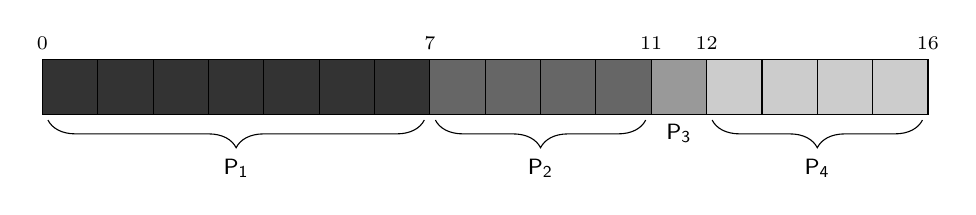
\begin{tikzpicture}

        \fill [black!80] (0,0) rectangle (14em, 2em);

        \fill [black!60] (14em,0) rectangle (22em, 2em);

        \fill [black!40] (22em,0) rectangle (24em, 2em);

        \fill [black!20] (24em,0) rectangle (32em, 2em);

        \draw (0,0) rectangle (32em,2em);

        \foreach \i in {1,...,15} {
          \draw [shorten >=0] (\i * 2em, 0) -- (\i * 2em, 2em);
        }

        \node [anchor=south] at (0em, 2em) {\scriptsize 0};
        \node [anchor=south] at (14em, 2em) {\scriptsize 7};
        \node [anchor=south] at (22em, 2em) {\scriptsize 11};
        \node [anchor=south] at (24em, 2em) {\scriptsize 12};
        \node [anchor=south] at (32em, 2em) {\scriptsize 16};

        \draw [decorate, decoration={brace,amplitude=10pt,mirror,raise=2pt}]
              (0.2em,0) -- (13.8em,0)
              node [midway, below, anchor=north, yshift=-1.25em]
              {\footnotesize $\mathsf{P_1}$};

        \draw [decorate, decoration={brace,amplitude=10pt,mirror,raise=2pt}]
              (14.2em,0) -- (21.8em,0)
              node [midway, below, anchor=north, yshift=-1.25em]
              {\footnotesize $\mathsf{P_2}$};

        \node [anchor=north] at (23em, 0) {\footnotesize $\mathsf{P_3}$};

        \draw [decorate, decoration={brace,amplitude=10pt,mirror,raise=2pt}]
              (24.2em,0) -- (31.8em,0)
              node [midway, below, anchor=north, yshift=-1.25em]
              {\footnotesize $\mathsf{P_4}$};
      \end{tikzpicture}
    \end{center}

    What is the average waiting time?
  \end{slide}
  
  \begin{slide}
    \slidetitle{What Happens to Our Waiting Time with a Different Arrival Order}

    Consider the same processes:

    \begin{center}
      \footnotesize
      \begin{tabular}{lrr}
        Process & Arrival Time & Burst Time \\
        $\mathsf{P_1}$ & 0 & 7 \\
        $\mathsf{P_2}$ & 0 & 4 \\
        $\mathsf{P_3}$ & 0 & 1 \\
        $\mathsf{P_4}$ & 0 & 4 \\
      \end{tabular}
    \end{center}
    \medskip

    Assume, $\mathsf{P_3} \rightarrow \mathsf{P_2} \rightarrow \mathsf{P_4}
             \rightarrow \mathsf{P_1}$.
    For FCFS, our schedule is:

    \begin{center}
      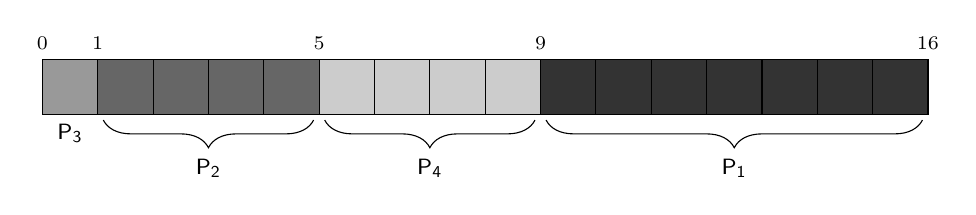
\begin{tikzpicture}

        \fill [black!80] (18em,0) rectangle (32em, 2em);

        \fill [black!60] (2em,0) rectangle (10em, 2em);

        \fill [black!40] (0em,0) rectangle (2em, 2em);

        \fill [black!20] (10em,0) rectangle (18em, 2em);

        \draw (0,0) rectangle (32em,2em);

        \foreach \i in {1,...,15} {
          \draw [shorten >=0] (\i * 2em, 0) -- (\i * 2em, 2em);
        }

        \node [anchor=south] at (0em, 2em) {\scriptsize 0};
        \node [anchor=south] at (2em, 2em) {\scriptsize 1};
        \node [anchor=south] at (10em, 2em) {\scriptsize 5};
        \node [anchor=south] at (18em, 2em) {\scriptsize 9};
        \node [anchor=south] at (32em, 2em) {\scriptsize 16};

        \node [anchor=north] at (1em, 0) {\footnotesize $\mathsf{P_3}$};

        \draw [decorate, decoration={brace,amplitude=10pt,mirror,raise=2pt}]
              (18.2em,0) -- (31.8em,0)
              node [midway, below, anchor=north, yshift=-1.25em]
              {\footnotesize $\mathsf{P_1}$};

        \draw [decorate, decoration={brace,amplitude=10pt,mirror,raise=2pt}]
              (2.2em,0) -- (9.8em,0)
              node [midway, below, anchor=north, yshift=-1.25em]
              {\footnotesize $\mathsf{P_2}$};

        \draw [decorate, decoration={brace,amplitude=10pt,mirror,raise=2pt}]
              (10.2em,0) -- (17.8em,0)
              node [midway, below, anchor=north, yshift=-1.25em]
              {\footnotesize $\mathsf{P_4}$};
      \end{tikzpicture}
    \end{center}

    What is the average waiting time now?
  \end{slide}

  \begin{slide}

    \slidetitle{Shortest Job First (SJF)}

    A slight tweak to FCFS, we always schedule the job with the shortest burst time
    first
    \medskip

    We're still assuming no preemption

  \end{slide}

  \begin{slide}

    \slidetitle{SJF Minimizes the Average Wait Time over FCFS}

    Consider the same processes with different arrival times:

    \begin{center}
      \footnotesize
      \begin{tabular}{lrr}
        Process & Arrival Time & Burst Time \\
        $\mathsf{P_1}$ & 0 & 7 \\
        $\mathsf{P_2}$ & 2 & 4 \\
        $\mathsf{P_3}$ & 4 & 1 \\
        $\mathsf{P_4}$ & 5 & 4 \\
      \end{tabular}
    \end{center}

    For SJF, our schedule is (arrival on top):

    \begin{center}
      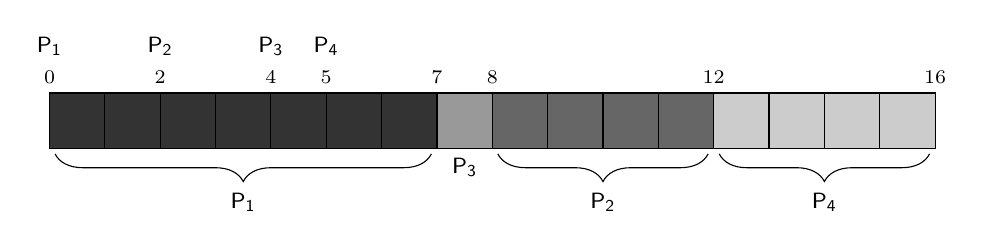
\begin{tikzpicture}

        \fill [black!80] (0,0) rectangle (14em, 2em);

        \fill [black!60] (16em,0) rectangle (24em, 2em);

        \fill [black!40] (14em,0) rectangle (16em, 2em);

        \fill [black!20] (24em,0) rectangle (32em, 2em);

        \draw (0,0) rectangle (32em,2em);

        \foreach \i in {1,...,15} {
          \draw [shorten >=0] (\i * 2em, 0) -- (\i * 2em, 2em);
        }

        \node [anchor=south] at (0em, 2em) {\scriptsize 0};
        \node [anchor=south] at (4em, 2em) {\scriptsize 2};
        \node [anchor=south] at (8em, 2em) {\scriptsize 4};
        \node [anchor=south] at (10em, 2em) {\scriptsize 5};
        \node [anchor=south] at (14em, 2em) {\scriptsize 7};
        \node [anchor=south] at (16em, 2em) {\scriptsize 8};
        \node [anchor=south] at (24em, 2em) {\scriptsize 12};
        \node [anchor=south] at (32em, 2em) {\scriptsize 16};

        \draw [decorate, decoration={brace,amplitude=10pt,mirror,raise=2pt}]
              (0.2em,0) -- (13.8em,0)
              node [midway, below, anchor=north, yshift=-1.25em]
              {\footnotesize $\mathsf{P_1}$};

        \draw [decorate, decoration={brace,amplitude=10pt,mirror,raise=2pt}]
              (16.2em,0) -- (23.8em,0)
              node [midway, below, anchor=north, yshift=-1.25em]
              {\footnotesize $\mathsf{P_2}$};

        \node [anchor=north] at (15em, 0) {\footnotesize $\mathsf{P_3}$};

        \draw [decorate, decoration={brace,amplitude=10pt,mirror,raise=2pt}]
              (24.2em,0) -- (31.8em,0)
              node [midway, below, anchor=north, yshift=-1.25em]
              {\footnotesize $\mathsf{P_4}$};

        \node [anchor=south, yshift=1em] at (0em, 2em) {\footnotesize $\mathsf{P_1}$};

        \node [anchor=south, yshift=1em] at (4em, 2em) {\footnotesize $\mathsf{P_2}$};

        \node [anchor=south, yshift=1em] at (8em, 2em) {\footnotesize $\mathsf{P_3}$};

        \node [anchor=south, yshift=1em] at (10em, 2em) {\footnotesize $\mathsf{P_4}$};
      \end{tikzpicture}
    \end{center}

    Average waiting time: $\mathsf{\frac{0 + 6 + 3 + 7}{4} = 4}$

  \end{slide}

  \begin{slide}

    \slidetitle{SJF is Not Practical}

    It is provably optimal at minimizing average wait time (if no preemption)
    \medskip

    You will not know the burst times of each process

    \leftspace{}You could use the past to predict future executions
    \medskip

    You may starve long jobs (they may never execute)

  \end{slide}

  \begin{slide}

    \slidetitle{Shortest Remaining Time First (SRTF)}

    Changing SJF to run with preemptions requires another tweak
    \medskip

    We'll assume that our minimum execution time is one unit
    \medskip

    Similar to SJF, this optimizes the average waiting time

  \end{slide}

  \begin{slide}

    \slidetitle{SRTF Reduces the Average Wait Time Compared to SJF}

    Consider the same processes and arrival times as SJF:

    \begin{center}
      \footnotesize
      \begin{tabular}{lrr}
        Process & Arrival Time & Burst Time \\
        $\mathsf{P_1}$ & 0 & 7 \\
        $\mathsf{P_2}$ & 2 & 4 \\
        $\mathsf{P_3}$ & 4 & 1 \\
        $\mathsf{P_4}$ & 5 & 4 \\
      \end{tabular}
    \end{center}

    For SRTF, our schedule is (arrival on top):

    \begin{center}
      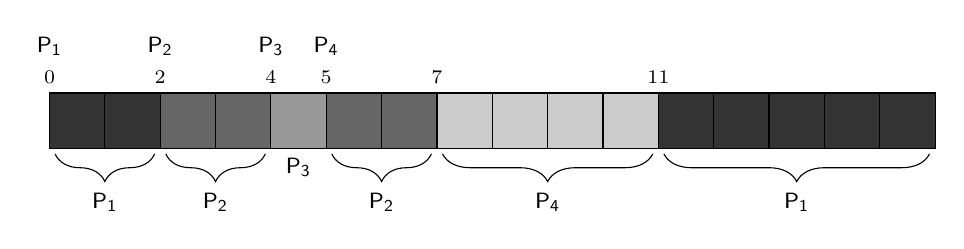
\begin{tikzpicture}

        \fill [black!80] (0,0) rectangle (4em, 2em);

        \fill [black!60] (4em,0) rectangle (8em, 2em);

        \fill [black!40] (8em,0) rectangle (10em, 2em);

        \fill [black!60] (10em,0) rectangle (14em, 2em);

        \fill [black!20] (14em,0) rectangle (22em, 2em);

        \fill [black!80] (22em,0) rectangle (32em, 2em);

        \draw (0,0) rectangle (32em,2em);

        \foreach \i in {1,...,15} {
          \draw [shorten >=0] (\i * 2em, 0) -- (\i * 2em, 2em);
        }

        \node [anchor=south] at (0em, 2em) {\scriptsize 0};
        \node [anchor=south] at (4em, 2em) {\scriptsize 2};
        \node [anchor=south] at (8em, 2em) {\scriptsize 4};
        \node [anchor=south] at (10em, 2em) {\scriptsize 5};
        \node [anchor=south] at (14em, 2em) {\scriptsize 7};
        \node [anchor=south] at (22em, 2em) {\scriptsize 11};

        \draw [decorate, decoration={brace,amplitude=10pt,mirror,raise=2pt}]
              (0.2em,0) -- (3.8em,0)
              node [midway, below, anchor=north, yshift=-1.25em]
              {\footnotesize $\mathsf{P_1}$};

        \draw [decorate, decoration={brace,amplitude=10pt,mirror,raise=2pt}]
              (4.2em,0) -- (7.8em,0)
              node [midway, below, anchor=north, yshift=-1.25em]
              {\footnotesize $\mathsf{P_2}$};

        \node [anchor=north] at (9em, 0) {\footnotesize $\mathsf{P_3}$};

        \draw [decorate, decoration={brace,amplitude=10pt,mirror,raise=2pt}]
              (10.2em,0) -- (13.8em,0)
              node [midway, below, anchor=north, yshift=-1.25em]
              {\footnotesize $\mathsf{P_2}$};

        \draw [decorate, decoration={brace,amplitude=10pt,mirror,raise=2pt}]
              (14.2em,0) -- (21.8em,0)
              node [midway, below, anchor=north, yshift=-1.25em]
              {\footnotesize $\mathsf{P_4}$};
              
        \draw [decorate, decoration={brace,amplitude=10pt,mirror,raise=2pt}]
              (22.2em,0) -- (31.8em,0)
              node [midway, below, anchor=north, yshift=-1.25em]
              {\footnotesize $\mathsf{P_1}$};

        \node [anchor=south, yshift=1em] at (0em, 2em) {\footnotesize $\mathsf{P_1}$};

        \node [anchor=south, yshift=1em] at (4em, 2em) {\footnotesize $\mathsf{P_2}$};

        \node [anchor=south, yshift=1em] at (8em, 2em) {\footnotesize $\mathsf{P_3}$};

        \node [anchor=south, yshift=1em] at (10em, 2em) {\footnotesize $\mathsf{P_4}$};
      \end{tikzpicture}
    \end{center}

    Average waiting time: $\mathsf{\frac{9 + 1 + 0 + 2}{4} = 3}$

  \end{slide}

  \begin{slide}

    \slidetitle{Round-Robin (RR)}

    So far we haven't handled fairness (it's a trade off with other metrics)
    \medskip

    The operating system divides execution into time slices (or quanta)

    \leftspace{}An individual time slice is called a quantum
    \medskip

    Maintain a FIFO queue of processes similar to FCFS

    \leftspace{}Preempt if still running at end of quantum and re-add to queue
    \medskip

    What are practical considerations for determining quantum length?

  \end{slide}

  \begin{slide}

    \slidetitle{RR with a Quantum Length of 3 Units}

    \begin{center}
      \footnotesize
      \begin{tabular}{lrr}
        Process & Arrival Time & Burst Time \\
        $\mathsf{P_1}$ & 0 & 7 \\
        $\mathsf{P_2}$ & 2 & 4 \\
        $\mathsf{P_3}$ & 4 & 1 \\
        $\mathsf{P_4}$ & 5 & 4 \\
      \end{tabular}
    \end{center}

    For RR, our schedule is (arrival on top, queue on bottom):

    \begin{center}
      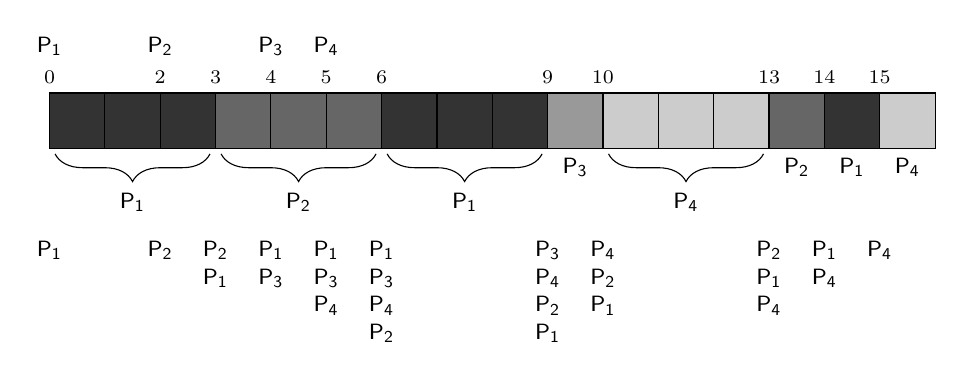
\begin{tikzpicture}

        \fill [black!80] (0,0) rectangle (6em, 2em);
        
        \fill [black!60] (6em,0) rectangle (12em, 2em);

        \fill [black!80] (12em,0) rectangle (18em, 2em);

        \fill [black!40] (18em,0) rectangle (20em, 2em);

        \fill [black!20] (20em,0) rectangle (26em, 2em);

        \fill [black!60] (26em,0) rectangle (28em, 2em);

        \fill [black!80] (28em,0) rectangle (30em, 2em);

        \fill [black!20] (30em,0) rectangle (32em, 2em);

        \draw (0,0) rectangle (32em,2em);

        \foreach \i in {1,...,15} {
          \draw [shorten >=0] (\i * 2em, 0) -- (\i * 2em, 2em);
        }

        \node [anchor=south] at (0em, 2em) {\scriptsize 0};
        \node [anchor=south] at (4em, 2em) {\scriptsize 2};
        \node [anchor=south] at (6em, 2em) {\scriptsize 3};
        \node [anchor=south] at (8em, 2em) {\scriptsize 4};
        \node [anchor=south] at (10em, 2em) {\scriptsize 5};
        \node [anchor=south] at (12em, 2em) {\scriptsize 6};
        \node [anchor=south] at (18em, 2em) {\scriptsize 9};
        \node [anchor=south] at (20em, 2em) {\scriptsize 10};
        \node [anchor=south] at (26em, 2em) {\scriptsize 13};
        \node [anchor=south] at (28em, 2em) {\scriptsize 14};
        \node [anchor=south] at (30em, 2em) {\scriptsize 15};

        \draw [decorate, decoration={brace,amplitude=10pt,mirror,raise=2pt}]
              (0.2em,0) -- (5.8em,0)
              node [midway, below, anchor=north, yshift=-1.25em]
              {\footnotesize $\mathsf{P_1}$};

        \draw [decorate, decoration={brace,amplitude=10pt,mirror,raise=2pt}]
              (6.2em,0) -- (11.8em,0)
              node [midway, below, anchor=north, yshift=-1.25em]
              {\footnotesize $\mathsf{P_2}$};

        \draw [decorate, decoration={brace,amplitude=10pt,mirror,raise=2pt}]
              (12.2em,0) -- (17.8em,0)
              node [midway, below, anchor=north, yshift=-1.25em]
              {\footnotesize $\mathsf{P_1}$};

        \node [anchor=north] at (19em, 0) {\footnotesize $\mathsf{P_3}$};

        \draw [decorate, decoration={brace,amplitude=10pt,mirror,raise=2pt}]
              (20.2em,0) -- (25.8em,0)
              node [midway, below, anchor=north, yshift=-1.25em]
              {\footnotesize $\mathsf{P_4}$};

        \node [anchor=north] at (27em, 0) {\footnotesize $\mathsf{P_2}$};

        \node [anchor=north] at (29em, 0) {\footnotesize $\mathsf{P_1}$};

        \node [anchor=north] at (31em, 0) {\footnotesize $\mathsf{P_4}$};

        \node [anchor=south, yshift=1em] at (0em, 2em) {\footnotesize $\mathsf{P_1}$};

        \node [anchor=south, yshift=1em] at (4em, 2em) {\footnotesize $\mathsf{P_2}$};

        \node [anchor=south, yshift=1em] at (8em, 2em) {\footnotesize $\mathsf{P_3}$};

        \node [anchor=south, yshift=1em] at (10em, 2em) {\footnotesize $\mathsf{P_4}$};

        \node [anchor=north, yshift=-3em] at (0em, 0em) {\footnotesize $\mathsf{P_1}$};

        \node [anchor=north, yshift=-3em] at (4em, 0em) {\footnotesize $\mathsf{P_2}$};

        \node [anchor=north, yshift=-3em] at (6em, 0em) {\footnotesize $\mathsf{P_2}$};
        \node [anchor=north, yshift=-4em] at (6em, 0em) {\footnotesize $\mathsf{P_1}$};

        \node [anchor=north, yshift=-3em] at (8em, 0em) {\footnotesize $\mathsf{P_1}$};
        \node [anchor=north, yshift=-4em] at (8em, 0em) {\footnotesize $\mathsf{P_3}$};

        \node [anchor=north, yshift=-3em] at (10em, 0em) {\footnotesize $\mathsf{P_1}$};
        \node [anchor=north, yshift=-4em] at (10em, 0em) {\footnotesize $\mathsf{P_3}$};
        \node [anchor=north, yshift=-5em] at (10em, 0em) {\footnotesize $\mathsf{P_4}$};

        \node [anchor=north, yshift=-3em] at (12em, 0em) {\footnotesize $\mathsf{P_1}$};
        \node [anchor=north, yshift=-4em] at (12em, 0em) {\footnotesize $\mathsf{P_3}$};
        \node [anchor=north, yshift=-5em] at (12em, 0em) {\footnotesize $\mathsf{P_4}$};
        \node [anchor=north, yshift=-6em] at (12em, 0em) {\footnotesize $\mathsf{P_2}$};

        \node [anchor=north, yshift=-3em] at (18em, 0em) {\footnotesize $\mathsf{P_3}$};
        \node [anchor=north, yshift=-4em] at (18em, 0em) {\footnotesize $\mathsf{P_4}$};
        \node [anchor=north, yshift=-5em] at (18em, 0em) {\footnotesize $\mathsf{P_2}$};
        \node [anchor=north, yshift=-6em] at (18em, 0em) {\footnotesize $\mathsf{P_1}$};

        \node [anchor=north, yshift=-3em] at (20em, 0em) {\footnotesize $\mathsf{P_4}$};
        \node [anchor=north, yshift=-4em] at (20em, 0em) {\footnotesize $\mathsf{P_2}$};
        \node [anchor=north, yshift=-5em] at (20em, 0em) {\footnotesize $\mathsf{P_1}$};

        \node [anchor=north, yshift=-3em] at (26em, 0em) {\footnotesize $\mathsf{P_2}$};
        \node [anchor=north, yshift=-4em] at (26em, 0em) {\footnotesize $\mathsf{P_1}$};
        \node [anchor=north, yshift=-5em] at (26em, 0em) {\footnotesize $\mathsf{P_4}$};

        \node [anchor=north, yshift=-3em] at (28em, 0em) {\footnotesize $\mathsf{P_1}$};
        \node [anchor=north, yshift=-4em] at (28em, 0em) {\footnotesize $\mathsf{P_4}$};

        \node [anchor=north, yshift=-3em] at (30em, 0em) {\footnotesize $\mathsf{P_4}$};
      \end{tikzpicture}
    \end{center}

  \end{slide}

  \begin{slide}

    \slidetitle{Metrics for RR (3 Unit Quantum Length)}

    Number of context switches: 7
    \medskip

    Average waiting time: $\mathsf{\frac{8 + 8 + 5 + 7}{4} = 7}$
    \medskip

    Average response time: $\mathsf{\frac{0 + 1 + 5 + 5}{4} = 2.75}$
    \bigskip

    Note: on ties (a new process arrives while one is preempted), favor the new one

  \end{slide}

  \begin{slide}

    \slidetitle{RR with a Quantum Length of 1 Units}

    \begin{center}
      \footnotesize
      \begin{tabular}{lrr}
        Process & Arrival Time & Burst Time \\
        $\mathsf{P_1}$ & 0 & 7 \\
        $\mathsf{P_2}$ & 2 & 4 \\
        $\mathsf{P_3}$ & 4 & 1 \\
        $\mathsf{P_4}$ & 5 & 4 \\
      \end{tabular}
    \end{center}

    For RR, our schedule is (arrival on top, queue on bottom):

    \begin{center}
      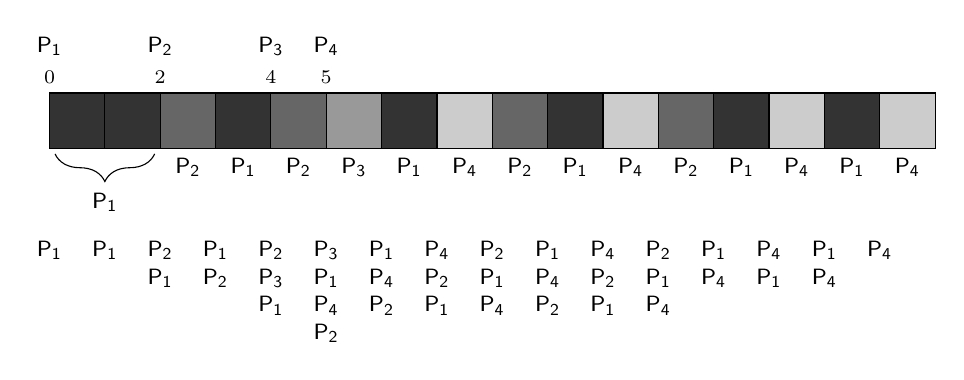
\begin{tikzpicture}

        \fill [black!80] (0,0) rectangle (4em, 2em);
        \fill [black!60] (4em,0) rectangle (6em, 2em);
        \fill [black!80] (6em,0) rectangle (8em, 2em);
        \fill [black!60] (8em,0) rectangle (10em, 2em);
        \fill [black!40] (10em,0) rectangle (12em, 2em);
        \fill [black!80] (12em,0) rectangle (14em, 2em);
        \fill [black!20] (14em,0) rectangle (16em, 2em);
        \fill [black!60] (16em,0) rectangle (18em, 2em);
        \fill [black!80] (18em,0) rectangle (20em, 2em);
        \fill [black!20] (20em,0) rectangle (22em, 2em);
        \fill [black!60] (22em,0) rectangle (24em, 2em);
        \fill [black!80] (24em,0) rectangle (26em, 2em);
        \fill [black!20] (26em,0) rectangle (28em, 2em);
        \fill [black!80] (28em,0) rectangle (30em, 2em);
        \fill [black!20] (30em,0) rectangle (32em, 2em);

        \draw (0,0) rectangle (32em,2em);

        \foreach \i in {1,...,15} {
          \draw [shorten >=0] (\i * 2em, 0) -- (\i * 2em, 2em);
        }

        \node [anchor=south] at (0em, 2em) {\scriptsize 0};
        \node [anchor=south] at (4em, 2em) {\scriptsize 2};
        \node [anchor=south] at (8em, 2em) {\scriptsize 4};
        \node [anchor=south] at (10em, 2em) {\scriptsize 5};

        \draw [decorate, decoration={brace,amplitude=10pt,mirror,raise=2pt}]
              (0.2em,0) -- (3.8em,0)
              node [midway, below, anchor=north, yshift=-1.25em]
              {\footnotesize $\mathsf{P_1}$};

        \node [anchor=north] at (5em, 0) {\footnotesize $\mathsf{P_2}$};
        \node [anchor=north] at (7em, 0) {\footnotesize $\mathsf{P_1}$};
        \node [anchor=north] at (9em, 0) {\footnotesize $\mathsf{P_2}$};
        \node [anchor=north] at (11em, 0) {\footnotesize $\mathsf{P_3}$};
        \node [anchor=north] at (13em, 0) {\footnotesize $\mathsf{P_1}$};
        \node [anchor=north] at (15em, 0) {\footnotesize $\mathsf{P_4}$};
        \node [anchor=north] at (17em, 0) {\footnotesize $\mathsf{P_2}$};
        \node [anchor=north] at (19em, 0) {\footnotesize $\mathsf{P_1}$};
        \node [anchor=north] at (21em, 0) {\footnotesize $\mathsf{P_4}$};
        \node [anchor=north] at (23em, 0) {\footnotesize $\mathsf{P_2}$};
        \node [anchor=north] at (25em, 0) {\footnotesize $\mathsf{P_1}$};
        \node [anchor=north] at (27em, 0) {\footnotesize $\mathsf{P_4}$};
        \node [anchor=north] at (29em, 0) {\footnotesize $\mathsf{P_1}$};
        \node [anchor=north] at (31em, 0) {\footnotesize $\mathsf{P_4}$};

        % Arrivals
        \node [anchor=south, yshift=1em] at (0em, 2em) {\footnotesize $\mathsf{P_1}$};
        \node [anchor=south, yshift=1em] at (4em, 2em) {\footnotesize $\mathsf{P_2}$};
        \node [anchor=south, yshift=1em] at (8em, 2em) {\footnotesize $\mathsf{P_3}$};
        \node [anchor=south, yshift=1em] at (10em, 2em) {\footnotesize $\mathsf{P_4}$};

        % Queues
        \node [anchor=north, yshift=-3em] at (0em, 0em) {\footnotesize $\mathsf{P_1}$};

        \node [anchor=north, yshift=-3em] at (2em, 0em) {\footnotesize $\mathsf{P_1}$};

        \node [anchor=north, yshift=-3em] at (4em, 0em) {\footnotesize $\mathsf{P_2}$};
        \node [anchor=north, yshift=-4em] at (4em, 0em) {\footnotesize $\mathsf{P_1}$};

        \node [anchor=north, yshift=-3em] at (6em, 0em) {\footnotesize $\mathsf{P_1}$};
        \node [anchor=north, yshift=-4em] at (6em, 0em) {\footnotesize $\mathsf{P_2}$};

        \node [anchor=north, yshift=-3em] at (8em, 0em) {\footnotesize $\mathsf{P_2}$};
        \node [anchor=north, yshift=-4em] at (8em, 0em) {\footnotesize $\mathsf{P_3}$};
        \node [anchor=north, yshift=-5em] at (8em, 0em) {\footnotesize $\mathsf{P_1}$};

        \node [anchor=north, yshift=-3em] at (10em, 0em) {\footnotesize $\mathsf{P_3}$};
        \node [anchor=north, yshift=-4em] at (10em, 0em) {\footnotesize $\mathsf{P_1}$};
        \node [anchor=north, yshift=-5em] at (10em, 0em) {\footnotesize $\mathsf{P_4}$};
        \node [anchor=north, yshift=-6em] at (10em, 0em) {\footnotesize $\mathsf{P_2}$};

        \node [anchor=north, yshift=-3em] at (12em, 0em) {\footnotesize $\mathsf{P_1}$};
        \node [anchor=north, yshift=-4em] at (12em, 0em) {\footnotesize $\mathsf{P_4}$};
        \node [anchor=north, yshift=-5em] at (12em, 0em) {\footnotesize $\mathsf{P_2}$};

        \node [anchor=north, yshift=-3em] at (14em, 0em) {\footnotesize $\mathsf{P_4}$};
        \node [anchor=north, yshift=-4em] at (14em, 0em) {\footnotesize $\mathsf{P_2}$};
        \node [anchor=north, yshift=-5em] at (14em, 0em) {\footnotesize $\mathsf{P_1}$};

        \node [anchor=north, yshift=-3em] at (16em, 0em) {\footnotesize $\mathsf{P_2}$};
        \node [anchor=north, yshift=-4em] at (16em, 0em) {\footnotesize $\mathsf{P_1}$};
        \node [anchor=north, yshift=-5em] at (16em, 0em) {\footnotesize $\mathsf{P_4}$};

        \node [anchor=north, yshift=-3em] at (18em, 0em) {\footnotesize $\mathsf{P_1}$};
        \node [anchor=north, yshift=-4em] at (18em, 0em) {\footnotesize $\mathsf{P_4}$};
        \node [anchor=north, yshift=-5em] at (18em, 0em) {\footnotesize $\mathsf{P_2}$};

        \node [anchor=north, yshift=-3em] at (20em, 0em) {\footnotesize $\mathsf{P_4}$};
        \node [anchor=north, yshift=-4em] at (20em, 0em) {\footnotesize $\mathsf{P_2}$};
        \node [anchor=north, yshift=-5em] at (20em, 0em) {\footnotesize $\mathsf{P_1}$};

        \node [anchor=north, yshift=-3em] at (22em, 0em) {\footnotesize $\mathsf{P_2}$};
        \node [anchor=north, yshift=-4em] at (22em, 0em) {\footnotesize $\mathsf{P_1}$};
        \node [anchor=north, yshift=-5em] at (22em, 0em) {\footnotesize $\mathsf{P_4}$};

        \node [anchor=north, yshift=-3em] at (24em, 0em) {\footnotesize $\mathsf{P_1}$};
        \node [anchor=north, yshift=-4em] at (24em, 0em) {\footnotesize $\mathsf{P_4}$};

        \node [anchor=north, yshift=-3em] at (26em, 0em) {\footnotesize $\mathsf{P_4}$};
        \node [anchor=north, yshift=-4em] at (26em, 0em) {\footnotesize $\mathsf{P_1}$};

        \node [anchor=north, yshift=-3em] at (28em, 0em) {\footnotesize $\mathsf{P_1}$};
        \node [anchor=north, yshift=-4em] at (28em, 0em) {\footnotesize $\mathsf{P_4}$};

        \node [anchor=north, yshift=-3em] at (30em, 0em) {\footnotesize $\mathsf{P_4}$};
      \end{tikzpicture}
    \end{center}

  \end{slide}

  \begin{slide}

    \slidetitle{Metrics for RR (1 Unit Quantum Length)}

    Number of context switches: 14
    \medskip

    Average waiting time: $\mathsf{\frac{8 + 6 + 1 + 7}{4} = 5.5}$
    \medskip

    Average response time: $\mathsf{\frac{0 + 0 + 1 + 2}{4} = 0.75}$

  \end{slide}

  \begin{slide}

    \slidetitle{RR with a Quantum Length of 10 Units}

    \begin{center}
      \footnotesize
      \begin{tabular}{lrr}
        Process & Arrival Time & Burst Time \\
        $\mathsf{P_1}$ & 0 & 7 \\
        $\mathsf{P_2}$ & 2 & 4 \\
        $\mathsf{P_3}$ & 4 & 1 \\
        $\mathsf{P_4}$ & 5 & 4 \\
      \end{tabular}
    \end{center}

    For RR, our schedule is (arrival on top, queue on bottom):

    \begin{center}
      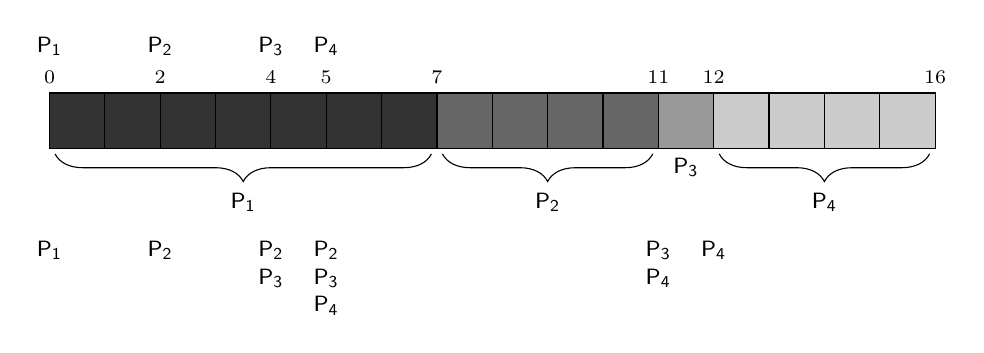
\begin{tikzpicture}

        \fill [black!80] (0,0) rectangle (14em, 2em);

        \fill [black!60] (14em,0) rectangle (22em, 2em);

        \fill [black!40] (22em,0) rectangle (24em, 2em);

        \fill [black!20] (24em,0) rectangle (32em, 2em);

        \draw (0,0) rectangle (32em,2em);

        \foreach \i in {1,...,15} {
          \draw [shorten >=0] (\i * 2em, 0) -- (\i * 2em, 2em);
        }

        \node [anchor=south] at (0em, 2em) {\scriptsize 0};
        \node [anchor=south] at (4em, 2em) {\scriptsize 2};
        \node [anchor=south] at (8em, 2em) {\scriptsize 4};
        \node [anchor=south] at (10em, 2em) {\scriptsize 5};
        \node [anchor=south] at (14em, 2em) {\scriptsize 7};
        \node [anchor=south] at (22em, 2em) {\scriptsize 11};
        \node [anchor=south] at (24em, 2em) {\scriptsize 12};
        \node [anchor=south] at (32em, 2em) {\scriptsize 16};

        % Arrivals
        \node [anchor=south, yshift=1em] at (0em, 2em) {\footnotesize $\mathsf{P_1}$};
        \node [anchor=south, yshift=1em] at (4em, 2em) {\footnotesize $\mathsf{P_2}$};
        \node [anchor=south, yshift=1em] at (8em, 2em) {\footnotesize $\mathsf{P_3}$};
        \node [anchor=south, yshift=1em] at (10em, 2em) {\footnotesize $\mathsf{P_4}$};

        % Queues
        \node [anchor=north, yshift=-3em] at (0em, 0em) {\footnotesize $\mathsf{P_1}$};

        \node [anchor=north, yshift=-3em] at (4em, 0em) {\footnotesize $\mathsf{P_2}$};

        \node [anchor=north, yshift=-3em] at (8em, 0em) {\footnotesize $\mathsf{P_2}$};
        \node [anchor=north, yshift=-4em] at (8em, 0em) {\footnotesize $\mathsf{P_3}$};

        \node [anchor=north, yshift=-3em] at (10em, 0em) {\footnotesize $\mathsf{P_2}$};
        \node [anchor=north, yshift=-4em] at (10em, 0em) {\footnotesize $\mathsf{P_3}$};
        \node [anchor=north, yshift=-5em] at (10em, 0em) {\footnotesize $\mathsf{P_4}$};

        \node [anchor=north, yshift=-3em] at (22em, 0em) {\footnotesize $\mathsf{P_3}$};
        \node [anchor=north, yshift=-4em] at (22em, 0em) {\footnotesize $\mathsf{P_4}$};

        \node [anchor=north, yshift=-3em] at (24em, 0em) {\footnotesize $\mathsf{P_4}$};


        \draw [decorate, decoration={brace,amplitude=10pt,mirror,raise=2pt}]
              (0.2em,0) -- (13.8em,0)
              node [midway, below, anchor=north, yshift=-1.25em]
              {\footnotesize $\mathsf{P_1}$};

        \draw [decorate, decoration={brace,amplitude=10pt,mirror,raise=2pt}]
              (14.2em,0) -- (21.8em,0)
              node [midway, below, anchor=north, yshift=-1.25em]
              {\footnotesize $\mathsf{P_2}$};

        \node [anchor=north] at (23em, 0) {\footnotesize $\mathsf{P_3}$};

        \draw [decorate, decoration={brace,amplitude=10pt,mirror,raise=2pt}]
              (24.2em,0) -- (31.8em,0)
              node [midway, below, anchor=north, yshift=-1.25em]
              {\footnotesize $\mathsf{P_4}$};
      \end{tikzpicture}
    \end{center}

  \end{slide}

  \begin{slide}

    \slidetitle{Metrics for RR (10 Unit Quantum Length)}

    Number of context switches: 3
    \medskip

    Average waiting time: $\mathsf{\frac{0 + 5 + 7 + 7}{4} = 4.75}$
    \medskip

    Average response time: $\mathsf{\frac{0 + 5 + 7 + 7}{4} = 4.75}$
    \bigskip

    Note: in this case it's the same as FCFS without preemptions

  \end{slide}

  \begin{slide}

    \slidetitle{RR Performance Depends on Quantum Length and Job Length}

    RR has low response good interactivity

    \leftspace{}Fair allocation of CPU

    \leftspace{}Low average waiting time (when job lengths vary)
    \bigskip

    The performance depends on the quantum length

    \leftspace{}Too high and it becomes FCFS

    \leftspace{}Too low and there's too many context switches (overhead)
    \medskip

    RR has poor average waiting time when jobs have similar lengths

  \end{slide}

  \begin{slide}

    \slidetitle{Scheduling Involves Trade-Offs}

    We looked at few different algorithms:

    \begin{itemize}
      \item First Come First Served (FCFS) is the most basic scheduling algorithm
      \item Shortest Job First (SJF) is a tweak that reduces waiting time
      \item Shortest Remaining Time First (SRTF) uses SJF ideas with preemptions
      \item SRTF optimizes lowest waiting time (or turnaround time)
      \item Round-robin (RR) optimizes fairness and response time
    \end{itemize}

  \end{slide}

\begin{slide}

	\slidetitle{Schedulers in real systems}
	
	Real schedulers are more complex
	\bigskip
	
	For example, Linux uses a Multi Level Feedback Queue (MLFQ)
	\begin{itemize}
		\item Many queues, in order of priority
		\item Process from highest priority queue scheduled first
		\item Within same priority, any algorithm like RR
		\item Priority of process decays with its age
	\end{itemize}

\end{slide}

\end{document}